\frame{
  \frametitle{Recozimento Simulado}
  \begin{block}{}
    \begin{figure}
      \centering
      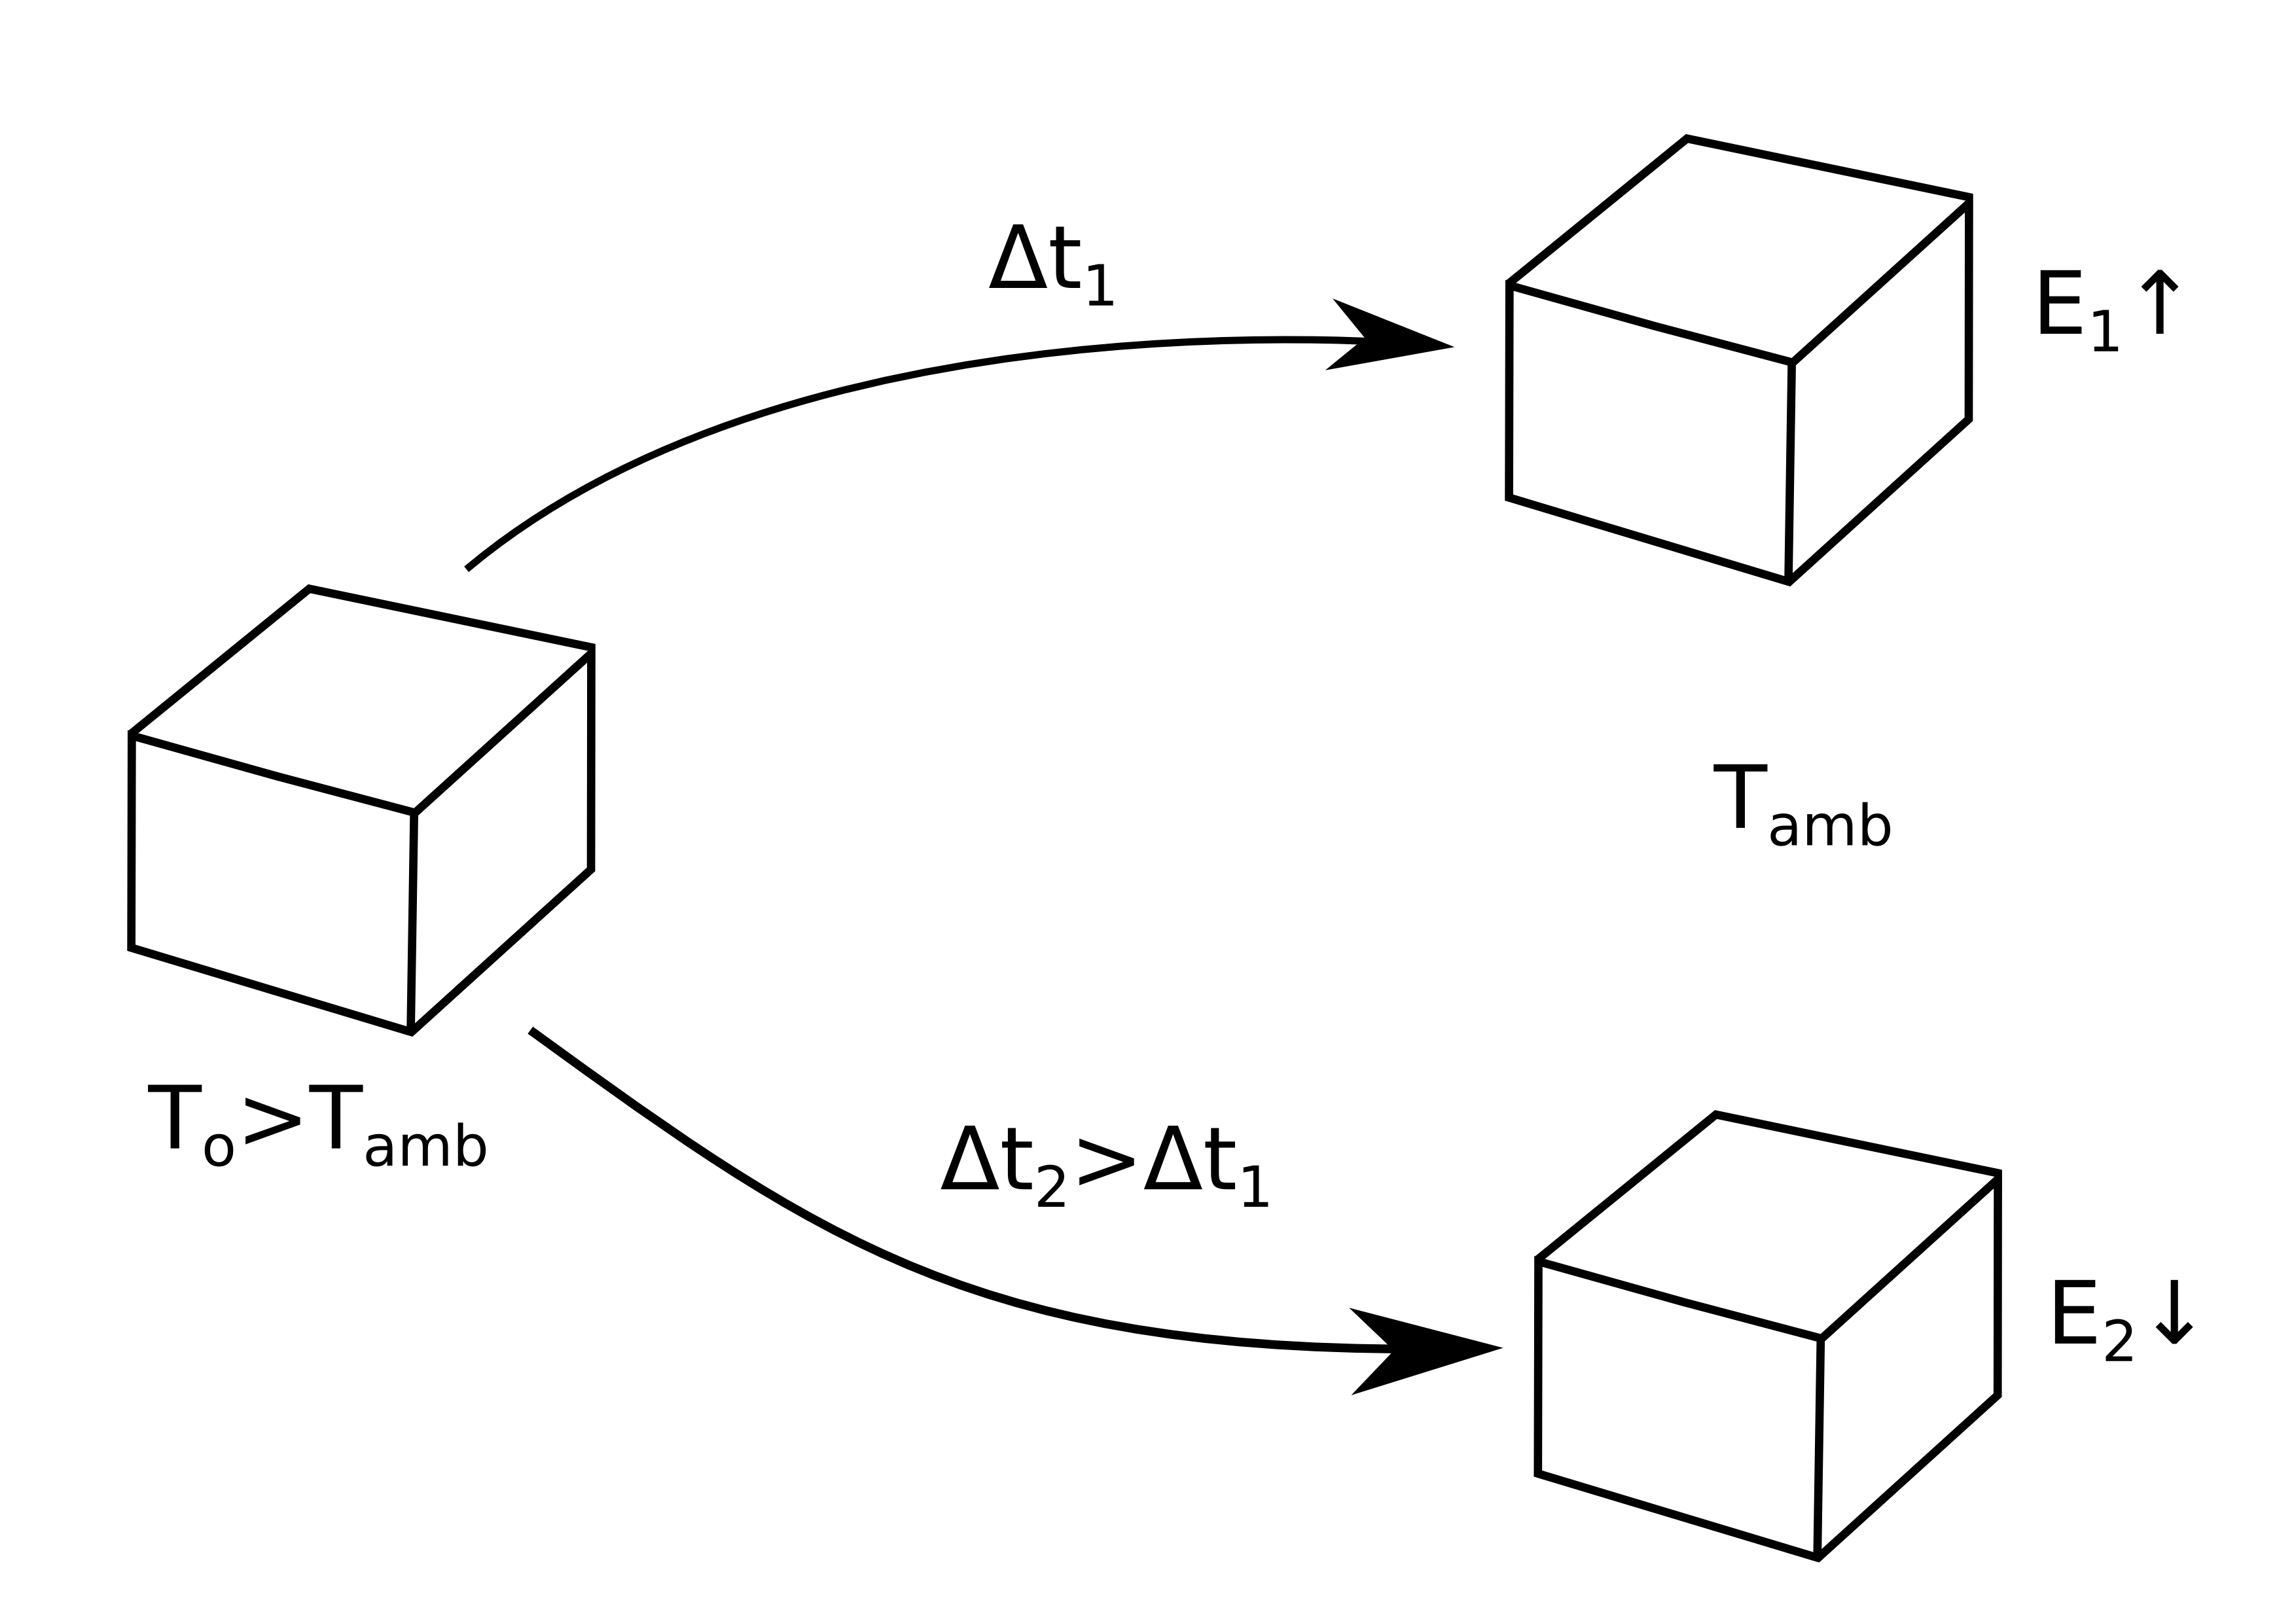
\includegraphics[width = 0.8 \linewidth]{imgs/ilustrativa_sa}
      \caption{Idéia Básica do SA}
    \end{figure}
  \end{block}
}

\frame{
  \frametitle{Recozimento Simulado}
  \begin{block}{}
    \begin{figure}
      \centering
      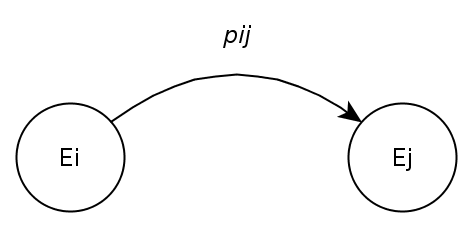
\includegraphics[width = 0.5 \linewidth]{imgs/transicao_sa}
      \caption{Probabilidade da Transição do Estado $i$ para o Estado $j$}
    \end{figure}
  \end{block}
  \begin{block}{}
    $$p_{ij}=\left\{\begin{array}{rc}
    1,&\mbox{se}\quad E\lbrace r_j \rbrace \le E\lbrace r_i \rbrace\\
    e^{\frac{- E\lbrace r_j \rbrace - E\lbrace r_i \rbrace}{k_B T} }, &\mbox{se}\quad 
    E\lbrace r_j \rbrace > E\lbrace r_i \rbrace
    \end{array}\right.
    $$
  \end{block}
}

\frame{
  \frametitle{Recozimento Simulado}
  \begin{block}{}
    Elementos básicos do SA:
    \begin{itemize}
      \item $S$ espaço de estado
      \item $J: S \rightarrow \mathbf{R}$, avalia os estados
      \item $S(i) \subset S - \lbrace i \rbrace$ para cada $i \in S$
      \item $q_{ij}, j \in S(i)$, tal que $\sum_{j \in S_{i}} q_{ij} = 1$
      \item $T$, função de resfriamento
      \item $x(0) \in S$, estado inicial
    \end{itemize}
  \end{block}
}